\secnumbersection{PROPUESTA DE SOLUCIÓN}

\subsection{Validación de Datos}

Típicamente una muestra a validar considera diez mil eventos por cada proceso de partículas individuales\footnote{Eventos simulados en los que se genera una única partícula inicial en una región específica del detector.} y colisiones\footnote{Eventos simulados en los que dos partículas colisionan, generando muchas otras partículas.}, al mismo tiempo se producen cerca de 110 mil eventos de partículas individuales y 250 mil de eventos de colisión, los cuales incluyen la aparición de muones, piones, electrones y procesos del modelo estándar. 
%
Antes de trabajar con estos datos, se debe determinar si son o no representativos, para lo cual se efectúa una \textit{validación de los datos}, compuesta de dos pasos: Primeramente, se pone a prueba el rendimiento del software utilizado para generar la simulación, y luego se testea el rendimiento desde el punto de vista de la física, comparando las simulaciones con datos empíricos \cite{Marshall2010}. 
%

El primer paso es, en su mayoría, realizado en forma de \emph{testings} automáticos y se basa en la búsqueda de \emph{bugs} que pudieran haber afectado la generación de los datos. 
%
El objetivo principal del segundo paso es determinar la calidad de la simulación a partir de análisis físicos y estadísticos sobre las muestras. Durante el presente trabajo se generó un algoritmo generador de histogramas con el propósito de representar los diferentes valores de las variables en cada región del detector.



%Se debe desarrollar la solución propuesta. Los subcapítulos por poner aquí son propios del autor. Se sugiere mencionar metodología usada. Es conveniente incorporar figuras y tablas para aclarar la solución, que deben indicar el número de la figura, su nombre y su autor o fuente (si las diseñas tú, la fuente es ``Elaboración propia''). Ver ejemplos en esta página y en la siguiente.

%Cabe mencionar que aquí está la esencia del trabajo en lo que se refiere al aporte creativo del memorista, es el momento de demostrar que usted es un destacado profesional que creó, diseñó y/o llevó a cabo la solución propuesta.

%\subsection{EJEMPLO DE COMO CITAR FIGURAS E ILUSTRACIONES}

%Se colocó una imagen que se puede referenciar también desde el texto (Ver figura \ref{fig:malla}).

%\begin{figure}[h]
%\centering
%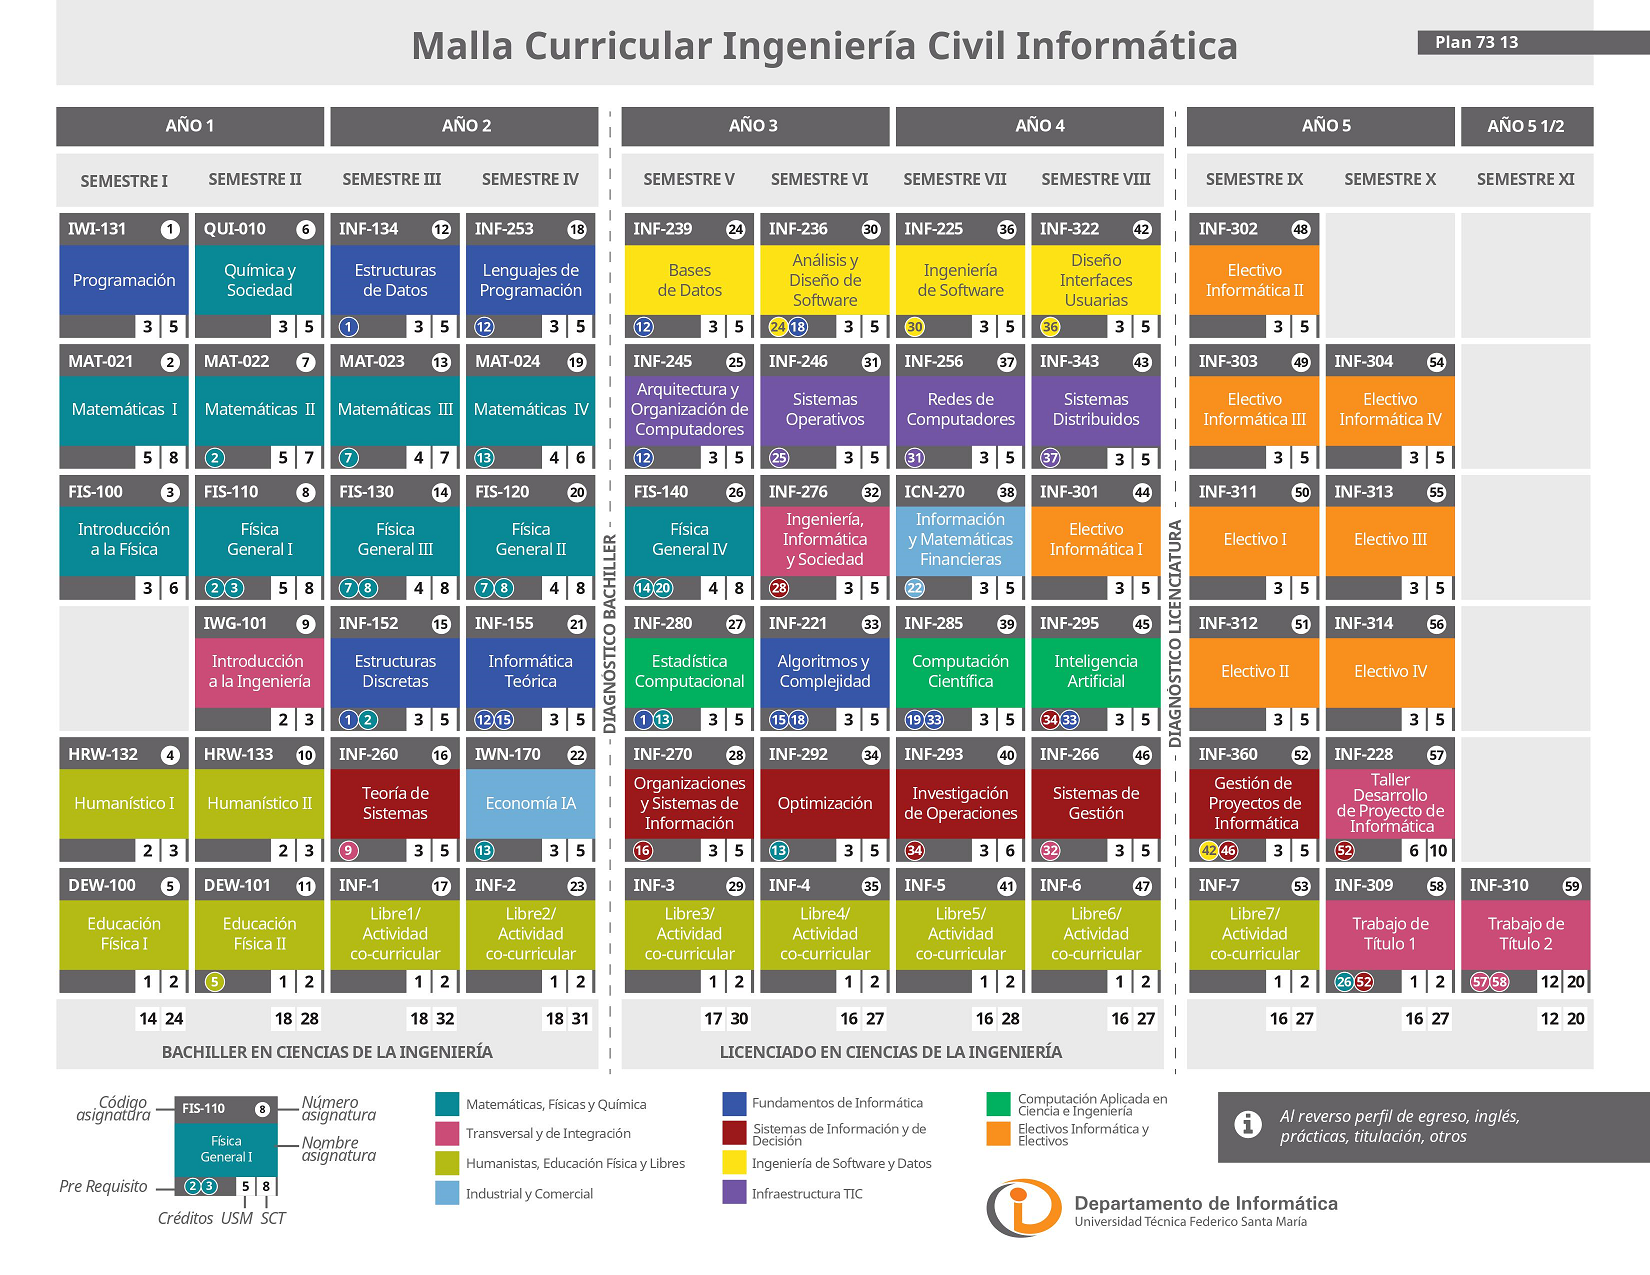
\includegraphics[width=0.8\textwidth]{malla_ingenieria_informatica}
%\caption{\label{fig:malla} Malla Curricular Ingeniería Civil Informática.} Fuente: Departamento de Informática.
%\end{figure}
